% XeLaTeX

\documentclass[a4paper]{article}
\usepackage{ctex}
\usepackage{xypic}
\usepackage{amsfonts,amssymb}
\usepackage{multirow}
\usepackage{geometry}
\usepackage{graphicx}
\usepackage{listings}
\usepackage{lipsum}
\usepackage{courier}
\usepackage{fancyvrb}
\usepackage{etoolbox}
\usepackage{longtable}


\linespread{1.2}
\geometry{left=3cm,right=2.5cm,top=2.5cm,bottom=2.5cm}

\makeatletter
\patchcmd{\FV@SetupFont}
  {\FV@BaseLineStretch}
  {\fontencoding{T1}\FV@BaseLineStretch}
  {}{}
\makeatother

\lstset{basicstyle=\small\fontencoding{T1}\ttfamily,breaklines=true}
\lstset{numbers=left,frame=shadowbox,tabsize=4}
%\lstset{extendedchars=false}
\begin{document}

\title{实验十 \ 文件服务 \ 实验报告}
\author {数据科学与计算机学院 \ 计算机科学与技术 2016 级 \\ 王凯祺 \ 16337233}
\maketitle

\section{实验目的}

\begin{itemize}
\item 学习文件操作的方法,掌握其实现方法。
\item 利用 FAT12 文件系统实现原型操作系统的文件管理控制命令。
\item 扩展 MyOS 的系统调用,实现进程中文件创建、文件打开、文件读、文件写和文件关闭等。
\end{itemize}

\section{实验要求}

原型保留原有特征的基础上,设计满足下列要求的新原型操作系统:

\begin{itemize}
\item 参考 DOS 的命令功能,实现文件管理控制命令 ls(目录显示) 、 rm(文件删除) 、cp(文件复制)、 cat(文件显示) 等。
\item 扩展 MyOS 的系统调用,在 C 语言中,程序可以调用文件创建、文件打开、文件读、文件写和文件关闭等系统调用。
\item 编写一个测试的这些系统调用的 C 语言用户程序,编译产生可执行程序进行测试。
\end{itemize}

\section{实验步骤}

\subsection{思路}

文件系统是个大工程。在做之前,要理清先做什么、后做什么,才能开始动手。

\begin{itemize}
\item 编写一个程序,用于测试中断调用的功能;
\item 分配一个中断号用于文件服务;
\item 设计共享的内核数据结构;
\item 实现文件服务中断的各功能;
\item 加入缓冲区功能。
\end{itemize}

\subsection{编写测试程序}

早期的测试程序是这样的:

\begin{lstlisting}[language=C]
int fopen(const char *filename, const char *type) {
	int t1, t2;
	t1 = filename;
	t2 = type;
	asm mov bx, t1
	asm mov cx, t2
	asm mov dx, ds
	asm mov ah, 0h
	asm int 26h
}

int fgetbyte(int f_id, unsigned char *w) {
	int t = w;
	asm mov bx, f_id
	asm mov cx, t
	asm mov dx, ds
	asm mov ah, 1h
	asm int 26h
}

char fgetc(int f_id) {
	unsigned char w;
	int ret;
	ret = fgetbyte(f_id, &w);
	if (ret < 0) return -1;
	return w;
}

void fputbyte(int f_id, unsigned char w) {
	asm mov bx, f_id
	asm mov ah, 2h
	asm mov al, w
	asm int 26h
}

void fputc(int f_id, char w) {
	fputbyte(f_id, w);
}

void fclose(int f_id) {
	asm mov bx, f_id
	asm mov ah, 3h
	asm int 26h
}
\end{lstlisting}

\begin{lstlisting}[language=C]
// main.cpp

#include "stdlib.h"
#include "stdio.h"
#include "file.h"

void main() {
	char src[20];
	char w;
	int f_src;
	src[0] = 'a'; src[1] = 'b'; src[2] = 'c'; src[3] = '.'; src[4] = 't'; src[5] = 'x'; src[6] = 't'; src[7] = 0;
	f_src = fopen(src, "r");
	if (f_src >= 0) {
	} else
	if (f_src == -1) {
		puts("error: file not found");
		exit(0);
	} else
	if (f_src == -2) {
		puts("error: file is being occupied");
		exit(0);
	} else
	if (f_src == -3) {
		puts("error: no enough space");
		exit(0);
	} else
	if (f_src == -4) {
		puts("error: unknown open method");
		exit(0);
	} else {
		puts("error: unknown error");
		exit(0);
	}
	while ((w = fgetc(f_src)) != -1) {
		putchar(w);
	}
	puts("");
	fclose(f_src);
	exit(0);
}
\end{lstlisting}

这个程序用于显示 abc.txt 的文件内容。由于文件写操作会修改磁盘信息,在编写测试程序时,应先测试读操作,读操作没有问题后,才测试写操作。所以在早期的测试程序中,只有读操作。

\subsection{分配中断号}

我为文件服务中断分配了 25h 这个中断号,这个中断号下有 4 个功能号。

\begin{longtable}{|l|p{1.8cm}|p{1.8cm}|p{1.8cm}|p{1.8cm}|p{1.8cm}|p{1.8cm}|}
\hline
\multirow{2}*{功能号 (AH)} & \multirow{2}*{功能描述} & \multicolumn{4}{|c|}{输入} & \multicolumn{1}{|c|}{输出} \\
\cline{3-7}
~ & ~ & AL & BX & CX & DX & AX \\
\hline
0x00 & 文件打开,给定文件名和打开方式,返回文件号或者错误 & - & 文件名字符串起始地址偏移量 & 打开方式字符串起始地址偏移量 & 字符串段地址 & 非负整数为文件号,负数为错误代码 \\
\hline
0x01 & 取字符,给定文件号和字符存储地址,将字符写入指定地址 & - & 文件号 & 字符存储地址偏移量 & 字符存储地址段地址 & 错误代码 \\
\hline
0x02 & 写字符,给定文件号和待写入的字符,将字符写入文件 & 待写字符 & 文件号 & - & - & - \\
\hline
0x03 & 关闭文件 & - & 文件号 & - & - & - \\
\hline
\end{longtable}

\subsection{设计共享的内核数据结构}

文件数据结构要有两个,一个是全局文件表,一个是进程文件表。

全局文件表维护的是每个文件的打开数量,以首簇号作为唯一标识符。

进程文件表维护的是特定进程打开文件的信息,包括当前文件指针,当前读取/写入的大小。

\begin{lstlisting}[language=C]
typedef struct processFileTable {
	unsigned char valid;
	char method;
	int offset;
	int first_cluster;
	int size;
	int current_cluster; /* 0 - 0xFFF */
	int current_pointer; /* 0 - 0x200 */
	int current_size;
};

typedef struct globalFileTable {
	unsigned char valid;
	char method;
	int first_cluster;
	int count;
};
\end{lstlisting}

\subsection{实现文件服务中断的各功能}

这部分是最难的,要实现读盘、写盘、读取下一簇簇号、改写下一簇簇号、寻找下一可用簇号等函数,才能实现文件服务中断的 4 个功能。

我在这里遇到的问题包括但不仅限于:

\begin{itemize}
\item C 语言中的指针传递问题
\item RC 问题
\item C 语言中的运算符优先级问题
\end{itemize}

\paragraph{C 语言中的指针传递问题}

考虑以下两段代码:

\begin{lstlisting}[language=C]
void b(char *st) {
	*st = 'a';
}

char st[N];
void a() {
	b(st);
	putchar(st[0]);
}
\end{lstlisting}

\begin{lstlisting}[language=C]
void b(char *st) {
	*st = 'a';
}

void a() {
	char st[N];
	b(st);
	putchar(st[0]);
}
\end{lstlisting}

第一段代码可以输出字符 'a' ,但第二段代码输出空字符。这是非常奇怪的事情!我用了多年的 gcc, g++ ,从来没在这个事情上栽过,结果一用 tcc ,各种 bug 就出来了?

把这两段代码都在 bochsdbg 跑一下,结果发现:

我们把 b(char *st) 函数进行汇编,结果如下:

\begin{lstlisting}[language={[x86masm]Assembler}]
	mov	bx, word ptr [bp+4]
	mov	byte ptr ds:[bx], 97
\end{lstlisting}

而第一段代码中 st[N] 是存放在 ds 段中, 第二段代码中 st[N] 是存放在 ss 段中。当 ds 段和 ss 段不一致时,传递指针就会出问题。

因此,我提供了一种解决方案,修改 b 函数的参数,添加 st 所在的段。

\begin{lstlisting}[language=C]
void b(char *st, unsigned int seg) {
	asm push ds
	asm mov ax, seg
	asm mov ds, ax
	*st = 'a';
	asm pop ds
}
\end{lstlisting}

加入段这个参数之后,两段代码均能正确执行。

\newpage

\paragraph{RC 问题}

我创建了 abc.txt 并运行刚刚编写的测试程序,结果如下:

\begin{figure}[!hbp]
\centering
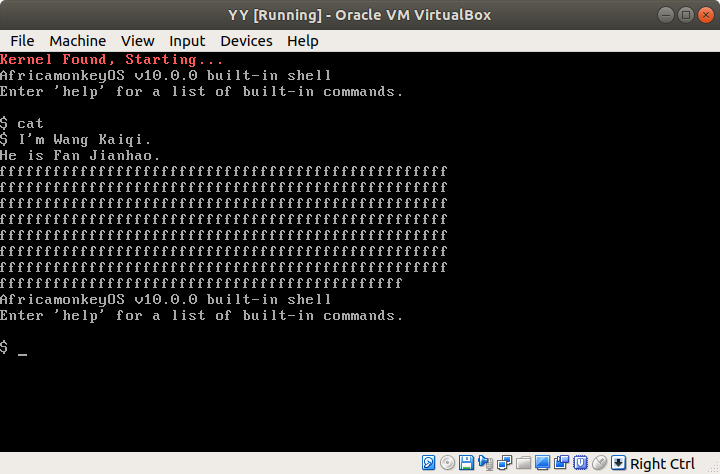
\includegraphics[scale=.5]{pics/1.png}
\end{figure}

\begin{figure}[!hbp]
\centering
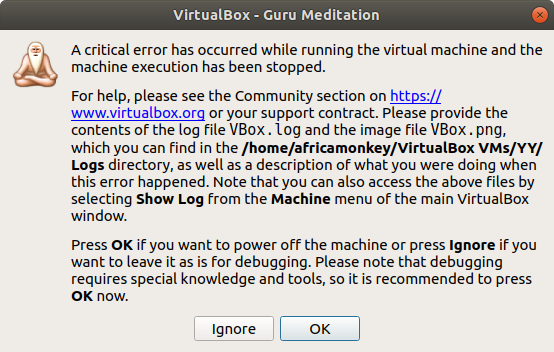
\includegraphics[scale=.5]{pics/2.png}
\end{figure}



从结果我们可以看出,程序输出到一半就崩溃了,还影响到了内核进程。

在文件服务中断中,为了避免 RC 问题,我使用了 cli 关闭中断,等文件服务结束后再通过 sti 打开中断。我还多此一举地使用信号量来保护 FAT 和全局文件表。如果关中断和使用信号量使用任意一个都是没有问题的,而我偏偏两个一起使用了,就出问题了。

我们还原一下文件服务中断的调用过程,首先由用户程序调用 26h 中断,文件中断响应后,调用 cli 关闭中断,执行到信号量相关代码时,由内核\textbf{调用 25h 中断} 。信号量中断响应后,调用 cli 关闭中断,执行一段代码后,\textbf{调用 sti 打开中断} 。返回文件服务中断时,中断是呈\textbf{开启}状态的。由此引发 RC 问题。

我将文件服务中断改成不需关中断,增加了一些信号量解决互斥问题,输出就正常了。

\paragraph{C 语言中的运算符优先级问题}

读取文件的测试完成了。测试复制文件时,我发现复制后的文件打不开,问题一定是出在写入文件上。我输出了调试信息,得到如下信息:

首簇号为 8 ,申请下一簇号为 9 ;

簇号 9,申请下一簇号为 10 ;

簇号 10,申请下一簇号为 9 。

为什么簇号 9 被占用了,簇号 10 还能申请到 9 这个编号呢???

我怀疑是簇号 9 没有正确地写入被占用的信息。事实证明我是对的:

原先我的 C 代码是这样的:

\begin{lstlisting}[language=C]
	if (current_cluster & 1) {
		a = ((int)a & 0x0f) | (val & 0x0f << 4);
		b = val >> 4;
	} else {
		a = val & 0xff;
		b = ((int)b & 0xf0) | (val >> 8);
	}
\end{lstlisting}

其中 current\_cluster 表示要修改的簇,val 表示修改的值。注意到上面的第 2 行,我以为 val \& 0x0f << 4 是从左到右进行运算的,谁知移位运算的优先级比与或优先级都要高。我在 val \& 0x0f 两侧加上括号,复制后的文件就能正常打开了。

\subsection{加入缓冲区功能}

我的代码原先是这样工作的:

对于读字符操作,每次读取一个扇区的数据,取出指定的字符返回,丢弃其他全部字符。

对于写字符操作,每次读取一个扇区的数据,改写指定的字符,再把整个扇区的字符写回。

如此操作的话,如果需要读/写 $x$ 字节的数据,则磁盘实际将读写 $512x$ 字节的数据。为了提高运行速度,提高文件系统的吞吐量,我们引入缓冲区。引入缓冲区之后,工作机制将发生变化:

对于读字符操作,如果缓冲区内是这个扇区的数据,返回指定字符;否则加载指定扇区数据并返回。

对于写字符操作,如果缓冲区未满,将字符写入缓冲区;否则将缓冲区写入扇区并清空,再将字符写入缓冲区。特别注意文件关闭时,无论缓冲区是否已满,都必须将缓冲区全部写回扇区。

加入缓冲区功能后,读写速率显著增加。以前复制一个 1.5 KB 的文件需要大约 3 秒的时间,现在用肉眼几乎很难测出时间。

\newpage

\subsection{功能展示}

下面展示的是我编写的用户程序 ls.com ,用于显示根目录文件信息。

\begin{figure}[!hbp]
\centering
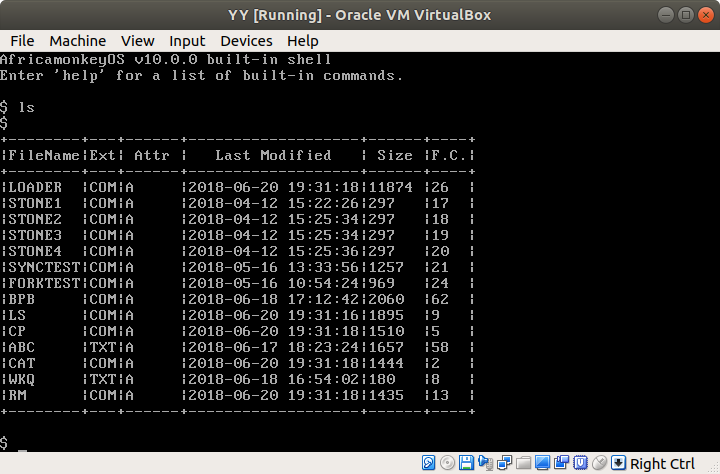
\includegraphics[scale=0.5]{pics/3.png}
\end{figure}

下面展示的是我编写的用户程序 cat.com ,用于显示文件内容。用法:cat file

\begin{figure}[!hbp]
\centering

\includegraphics[scale=0.5]{pics/4.png}
\end{figure}

\newpage

下面展示的是我编写的用户程序 cp.com ,用于文件复制。用法:cp filea fileb

\begin{figure}[!hbp]
\centering
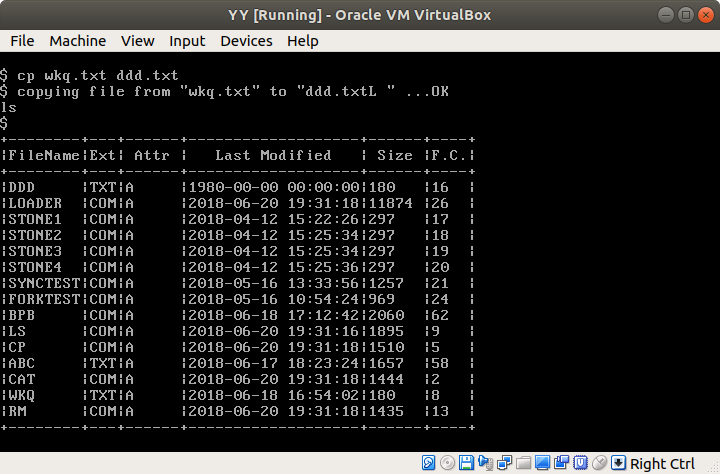
\includegraphics[scale=0.5]{pics/5.png}
\end{figure}

我们可以看到,根目录下多了一个文件 ddd.txt 。我们来看看 ddd.txt 的文件内容是否与 wkq.txt 一致。

\begin{figure}[!hbp]
\centering
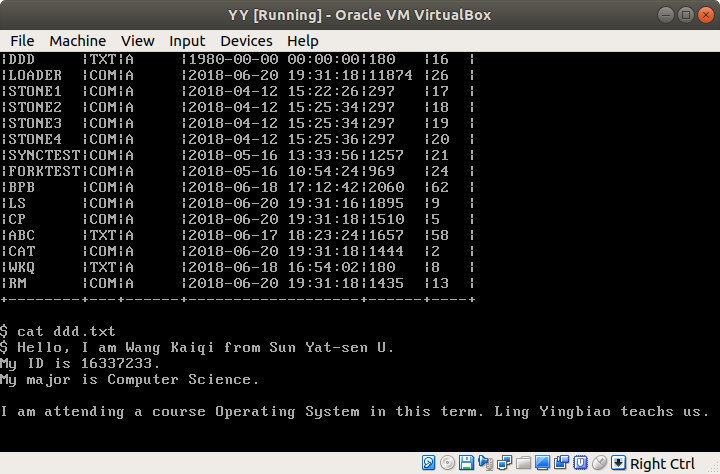
\includegraphics[scale=0.5]{pics/6.png}
\end{figure}

\newpage

下图展示的是我编写的用户程序 rm.com ,用于文件删除。用法: rm file

\begin{figure}[!hbp]
\centering
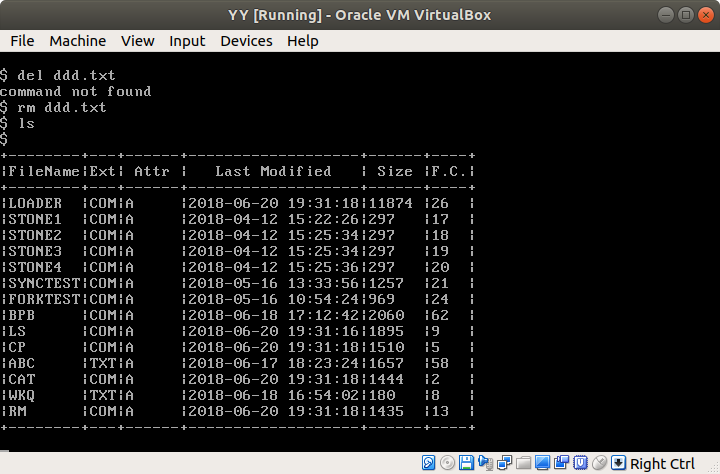
\includegraphics[scale=0.5]{pics/7.png}
\end{figure}

\section{实验总结}

写一个文件服务中断差不多用掉了半条命,用时大约两个星期……在此之前,内核的 C 代码只有 16 KB ;加了文件服务中断后,内核代码翻了一番,达到 33 KB 。

用时最多的当然是 debug 阶段,特别是查出问题根源的那个阶段。搜索文件时给定两个字符串(一个是主文件名,一个是扩展名),竟然发现其中一个能正确读取到字符,另一个不能读,最后定位到是 C 语言的指针传递问题是要靠我一步步通过 bochs 跟踪程序代码,一行行看汇编结果和堆栈情况,确定是哪个语句出问题。通过分析那个语句,得知参与计算的是 ds 而不是 ss 。

其次是思考从何入手的阶段,拿到 PPT 后发现才 6 页,只说了一些关键的细节。对整个项目先做什么、后做什么、怎么做,都是需要我思考的。比较让我困惑的是,如何处理字符串传递的问题。我们知道,用户程序在执行 fopen 时会传入一个字符串参数,表示文件名; shell 在执行用户程序时需要传参数(例如 cat file, cp file1 file2)。经过群里同学的提醒,我知道了可以通过将段和偏移地址保存在寄存器中,然后调用中断命令来传。后者(shell)我可不能这么干,因为这会产生 RC 问题:由于 shell 读取的字符串会被之后键盘输入覆盖,直接把 shell 读取的字符串的偏移地址传给用户程序是极其危险的事情,这相当于两个程序同时访问同一变量。所以我想了一个办法:参数保存在进程控制块(PCB)中,进程通过系统调用的方法将用户程序的一个字符串地址传给内核,由内核来将参数写到这个字符串地址。我真是太聪明啦!

\end{document}
















